%  ALWAYS USE THE referee OPTION WITH PAPERS SUBMITTED TO BIOMETRICS!!!
%  You can see what your paper would look like typeset by removing
%  the referee option.  Because the typeset version will be in two
%  columns, however, some of your equations may be too long. DO NOT
%  use the \longequation option discussed in the user guide!!!  This option
%  is reserved ONLY for equations that are impossible to split across 
%  multiple lines; e.g., a very wide matrix.  Instead, type your equations 
%  so that they stay in one column and are split across several lines, 
%  as are almost all equations in the journal.  Use a recent version of the
%  journal as a guide. 
%  
\documentclass[useAMS,referee]{biom}
\usepackage{amsmath}
\usepackage{graphicx}
\usepackage{blindtext}
\usepackage{booktabs}
\usepackage{breqn}
\usepackage{algorithm}
\usepackage{algcompatible}
\usepackage{algpseudocode}
\usepackage{float}
\usepackage{dutchcal}
\usepackage{amsfonts}




\let\origfigure\figure
\let\endorigfigure\endfigure
\renewenvironment{figure}[1][2] {
    \expandafter\origfigure\expandafter[H]
} {
    \endorigfigure
}


\def\bSig\mathbf{\Sigma}
\newcommand{\VS}{V\&S}
\newcommand{\tr}{\mbox{tr}}

%  Here, place your title and author information.  Note that in 
%  use of the \author command, you create your own footnotes.  Follow
%  the examples below in creating your author and affiliation information.
%  Also consult a recent issue of the journal for examples of formatting.

\title[]{Bayesian multivariate skew-normal finite mixture model for analysis of infant development trajectories}

%  Here are examples of different configurations of author/affiliation
%  displays.  According to the Biometrics style, in some instances,
%  the convention is to have superscript *, **, etc footnotes to indicate 
%  which of multiple email addresses belong to which author.  In this case,
%  use the \email{ } command to produce the emails in the display.

%  In other cases, such as a single author or two authors from 
%  different institutions, there should be no footnoting.  Here, use
%  the \emailx{ } command instead. 

%  The examples below corrspond to almost every possible configuration
%  of authors and may be used as a guide.  For other configurations, consult
%  a recent issue of the the journal.

%  Single author -- USE \emailx{ } here so that no asterisk footnoting
%  for the email address will be produced.

%\author{John Author\emailx{email@address.edu} \\
%Department of Statistics, University of Warwick, Coventry CV4 7AL, U.K.}

%  Two authors from the same institution, with both emails -- use
%  \email{ } here to produce the asterisk footnoting for each email address

%\author{John Author$^{*}$\email{author@address.edu} and
%Kathy Authoress$^{**}$\email{email2@address.edu} \\
%Department of Statistics, University of Warwick, Coventry CV4 7AL, U.K.}

%  Exactly two authors from different institutions, with both emails  
%  USE \emailx{ } here so that no asterisk footnoting for the email address
%  is produced.

\author
{Carter Allen\emailx{allecart@musc.edu} \\
Department of Public Health Sciences, Medical University of South Carolina, Charleston, SC, U.S.A
\and
Brian Neelon, PhD \\
Department of Public Health Sciences, Medical University of South Carolina, Charleston, SC, U.S.A
\and
Sara Benjamin-Neelon, PhD, MPH, RD \\
Department of Health, Behavior and Society, Johns Hopkins University, Baltimore, MD, U.S.A}

%  Three or more authors from same institution with all emails displayed
%  and footnoted using asterisks -- use \email{ } 

%\author{John Author$^*$\email{author@address.edu}, 
%Jane Author$^{**}$\email{jane@address.edu}, and 
%Dick Author$^{***}$\email{dick@address.edu} \\
%Department of Statistics, University of Warwick, Coventry CV4 7AL, U.K}

%  Three or more authors from same institution with one corresponding email
%  displayed

%\author{John Author$^*$\email{author@address.edu}, 
%Jane Author, and Dick Author \\
%Department of Statistics, University of Warwick, Coventry CV4 7AL, U.K}

%  Three or more authors, with at least two different institutions,
%  more than one email displayed 

%\author{John Author$^{1,*}$\email{author@address.edu}, 
%Kathy Author$^{2,**}$\email{anotherauthor@address.edu}, and 
%Wilma Flinstone$^{3,***}$\email{wilma@bedrock.edu} \\
%$^{1}$Department of Statistics, University of Warwick, Coventry CV4 7AL, U.K \\
%$^{2}$Department of Biostatistics, University of North Carolina at 
%Chapel Hill, Chapel Hill, North Carolina, U.S.A. \\
%$^{3}$Department of Geology, University of Bedrock, Bedrock, Kansas, U.S.A.}

%  Three or more authors with at least two different institutions and only
%  one email displayed

%\author{John Author$^{1,*}$\email{author@address.edu}, 
%Wilma Flinstone$^{2}$, and Barney Rubble$^{2}$ \\
%$^{1}$Department of Statistics, University of Warwick, Coventry CV4 7AL, U.K \\
%$^{2}$Department of Geology, University of Bedrock, Bedrock, Kansas, U.S.A.}


\begin{document}

%  This will produce the submission and review information that appears
%  right after the reference section.  Of course, it will be unknown when
%  you submit your paper, so you can either leave this out or put in 
%  sample dates (these will have no effect on the fate of your paper in the
%  review process!)

\date{{\it Received October} 2007. {\it Revised February} 2008.  {\it
Accepted March} 2008.}

%  These options will count the number of pages and provide volume
%  and date information in the upper left hand corner of the top of the 
%  first page as in published papers.  The \pagerange command will only
%  work if you place the command \label{firstpage} near the beginning
%  of the document and \label{lastpage} at the end of the document, as we
%  have done in this template.

%  Again, putting a volume number and date is for your own amusement and
%  has no bearing on what actually happens to your paper!  

\pagerange{\pageref{firstpage}--\pageref{lastpage}} 
\volume{64}
\pubyear{2008}
\artmonth{December}

%  The \doi command is where the DOI for your paper would be placed should it
%  be published.  Again, if you make one up and stick it here, it means 
%  nothing!

\doi{10.1111/j.1541-0420.2005.00454.x}

%  This label and the label ``lastpage'' are used by the \pagerange
%  command above to give the page range for the article.  You may have 
%  to process the document twice to get this to match up with what you 
%  expect.  When using the referee option, this will not count the pages
%  with tables and figures.  

\label{firstpage}

%  put the summary for your paper here

\begin{abstract}
In studies of infant motor development, a crucial research goal is the identification of latent clusters of infants who experience delayed development, as this is a known risk factor for adverse outcomes later in life. However, there are a number of statistical challenges in modeling infant development: the data are typically skewed, exhibit intermittent missingness, and are highly correlated across the repeated measurements collected during infancy. Using data from the Nurture study, a cohort of over 600 mother-infant pairs followed from pregnancy to 12 months postpartum, we develop a flexible Bayesian finite mixture model for the analysis infant motor development. Our model has a number of attractive features. First, we adopt the multivariate skew normal distribution with cluster-specific parameters that accommodate the inherent correlation and skewness in the data. Second, we model the cluster membership probabilities using a novel application of the P\'olya-Gamma data-augmentation scheme, thereby improving predictions of the cluster membership allocations. Lastly, we impute missing responses under the missing at random assumption by drawing from appropriate conditional multivariate skew  normal distributions. Bayesian inference is achieved through straightforward Gibbs sampling, and can be implemented in available software such as \texttt{R}.  Through simulation studies, we show that the proposed model yields improved inferences over models that ignore skewness. In addition, our imputation method yields improvements compared to conventional missing data methods, including multiple imputation and complete or available case analysis. When applied to Nurture data, we identified two distinct development clusters: one characterized by delayed “U-shaped” development and a higher percentage of male infants and another characterized by more steady development and a lower percentage of males. The clusters also differed in terms of key demographic variables, such as infant race and maternal pre-pregnancy body mass index. These findings can aid investigators in targeting interventions during this critical early-life developmental window.
\end{abstract}

%  Please place your key words in alphabetical order, separated
%  by semicolons, with the first letter of the first word capitalized,
%  and a period at the end of the list.
%

\begin{keywords}
Mixture of Experts, P\'olya-Gamma, Skew-Normal, Imputation, Latent Growth, Infant Development.
\end{keywords}

%  As usual, the \maketitle command creates the title and author/affiliations
%  display

\maketitle

\setcounter{tocdepth}{3}
\tableofcontents

\newpage

%  If you are using the referee option, a new page, numbered page 1, will
%  start after the summary and keywords.  The page numbers thus count the
%  number of pages of your manuscript in the preferred submission style.
%  Remember, ``Normally, regular papers exceeding 25 pages and Reader Reaction 
%  papers exceeding 12 pages in (the preferred style) will be returned to 
%  the authors without review. The page limit includes acknowledgements, 
%  references, and appendices, but not tables and figures. The page count does 
%  not include the title page and abstract. A maximum of six (6) tables or 
%  figures combined is often required.''

%  You may now place the substance of your manuscript here.  Please use
%  the \section, \subsection, etc commands as described in the user guide.
%  Please use \label and \ref commands to cross-reference sections, equations,
%  tables, figures, etc.
%
%  Please DO NOT attempt to reformat the style of equation numbering!
%  For that matter, please do not attempt to redefine anything!

\section{Introduction}
\label{s:intro}

\subsection{Infant Development Clustering}

Heterogeneity of treatment effects (HTE) (Lanza and Rhoades, 2013). 

\subsection{Existing Approaches}

Mixtures of multivariate non-symmetric distributions such as the multivariate skew-normal (MSN) distribution allow for the nuances of the marginal density to be captured with a more parsimonious set of mixture components. Mixtures of MSN distributions have been dealt with previously in a Bayesian context (Fr\"{u}hwirth-Schnatter \& Pyne, 2010 and others), however in these models, focus lies primary on marginal density estimation, and inference on the mixture components (i.e. clusters) is often not discussed. More recently, the mixtures of skew-$t$ factor analysis (MSTFA) model has been proposed for settings in which cluster-specific inference is of primary interest (Lin \textit{et al.} 2018). However, an important feature not included in the MSTFA is the ability to explain individual-level cluster membership as a function of covariates of interest. Additionally, the parameter estimation procedure proposed by Lin et al. for the MSTFA relies on a prohibitively complex EM algorithm and does not enjoy the inferential benefits of a Bayesian approach, including the ability to incorporate prior information into a model and make posterior probability statements. Our proposed model improves on these previous works by estimating parameters in a Bayesian framework as well as including the ability to fit a multinomial logit regression to cluster membership probabilities using a novel application of data augmentation with the P\'olya-Gamma distribution.

Polson et al. (2013) introduce a data augmentation scheme using the P\'olya-Gamma distribution which allows for sampling of multinomial regression parameters using straightforward Gibb's updates from Gaussian full conditional distributions. In addition to more convinient parameter estimation, the P\'olya-Gamma data augmentation method for logistic regression has the advantage of direct sampling from the posterior distributions of multinomial parameters. This approach avoids the need for approximations of the posterior distribution, thus yeilding more stable sampling, especially when the number of parameters approaches the number of observations (Polson et al., 2013). P\'olya-Gamma data augmentation for multinomial regression has not yet been applied to the analysis of longitudinally clustered data. 

A ubiquitous feature of repeated measures studies is loss of data due to intermittent missingness and attrition. In the Bayesian setting, the standard approach to dealing with missing data is to perform multiple imputation, whereby $m$ imputed data sets are generated from a specified imputation model. After $m$ complete data sets are obtained, parameter estimates are combined across each data set to produce a final set of parameter estimates (Gelman \textit{et al.} 2013). This approach is not only computationally burdensome, requiring storage and analysis of an $m \times n_{rows} \times n_{cols}$ data array in addition to multiplication of total model run time by a factor of $m$, but it has been shown to produce unreliable inferences (Zhou and Reiter, 2010). We instead include an ``online" imputation imputation step in our Gibbs sampling procedure, whereby missing outcomes are updated at each iteration. This approach greatly increases the number of opportunities for exploration of the missing data parameter space and avoids the multiplication of total run time and number of parameters.

\newpage

\section{Nurture Study}
\label{s:nurt}
\subsection{Baseline Demographics and Description of Variables}

\subsection{Statistical Challenges}

The analysis of infant development trends in the Nurture data presents a number of statistical challenges that motivate our proposed model. First, as depicted in Figure 1, the residuals from repeated measures models of Bayley composite scores exhibit skewness even after adjusting for covariates such as race, sex, and birthweight. This suggests that the assumption of conditional normality made by standard repeated measures models is violated, and a distinguishing feature of the data, skewness, is not being accounted for. 

\vspace{1mm}
\begin{figure}[h]
	\label{fig:skew_resids}
	\caption{The distribution of residuals in repeated measures regression model of Bayley composite scores adjusted for race and sex.}
	\centering
	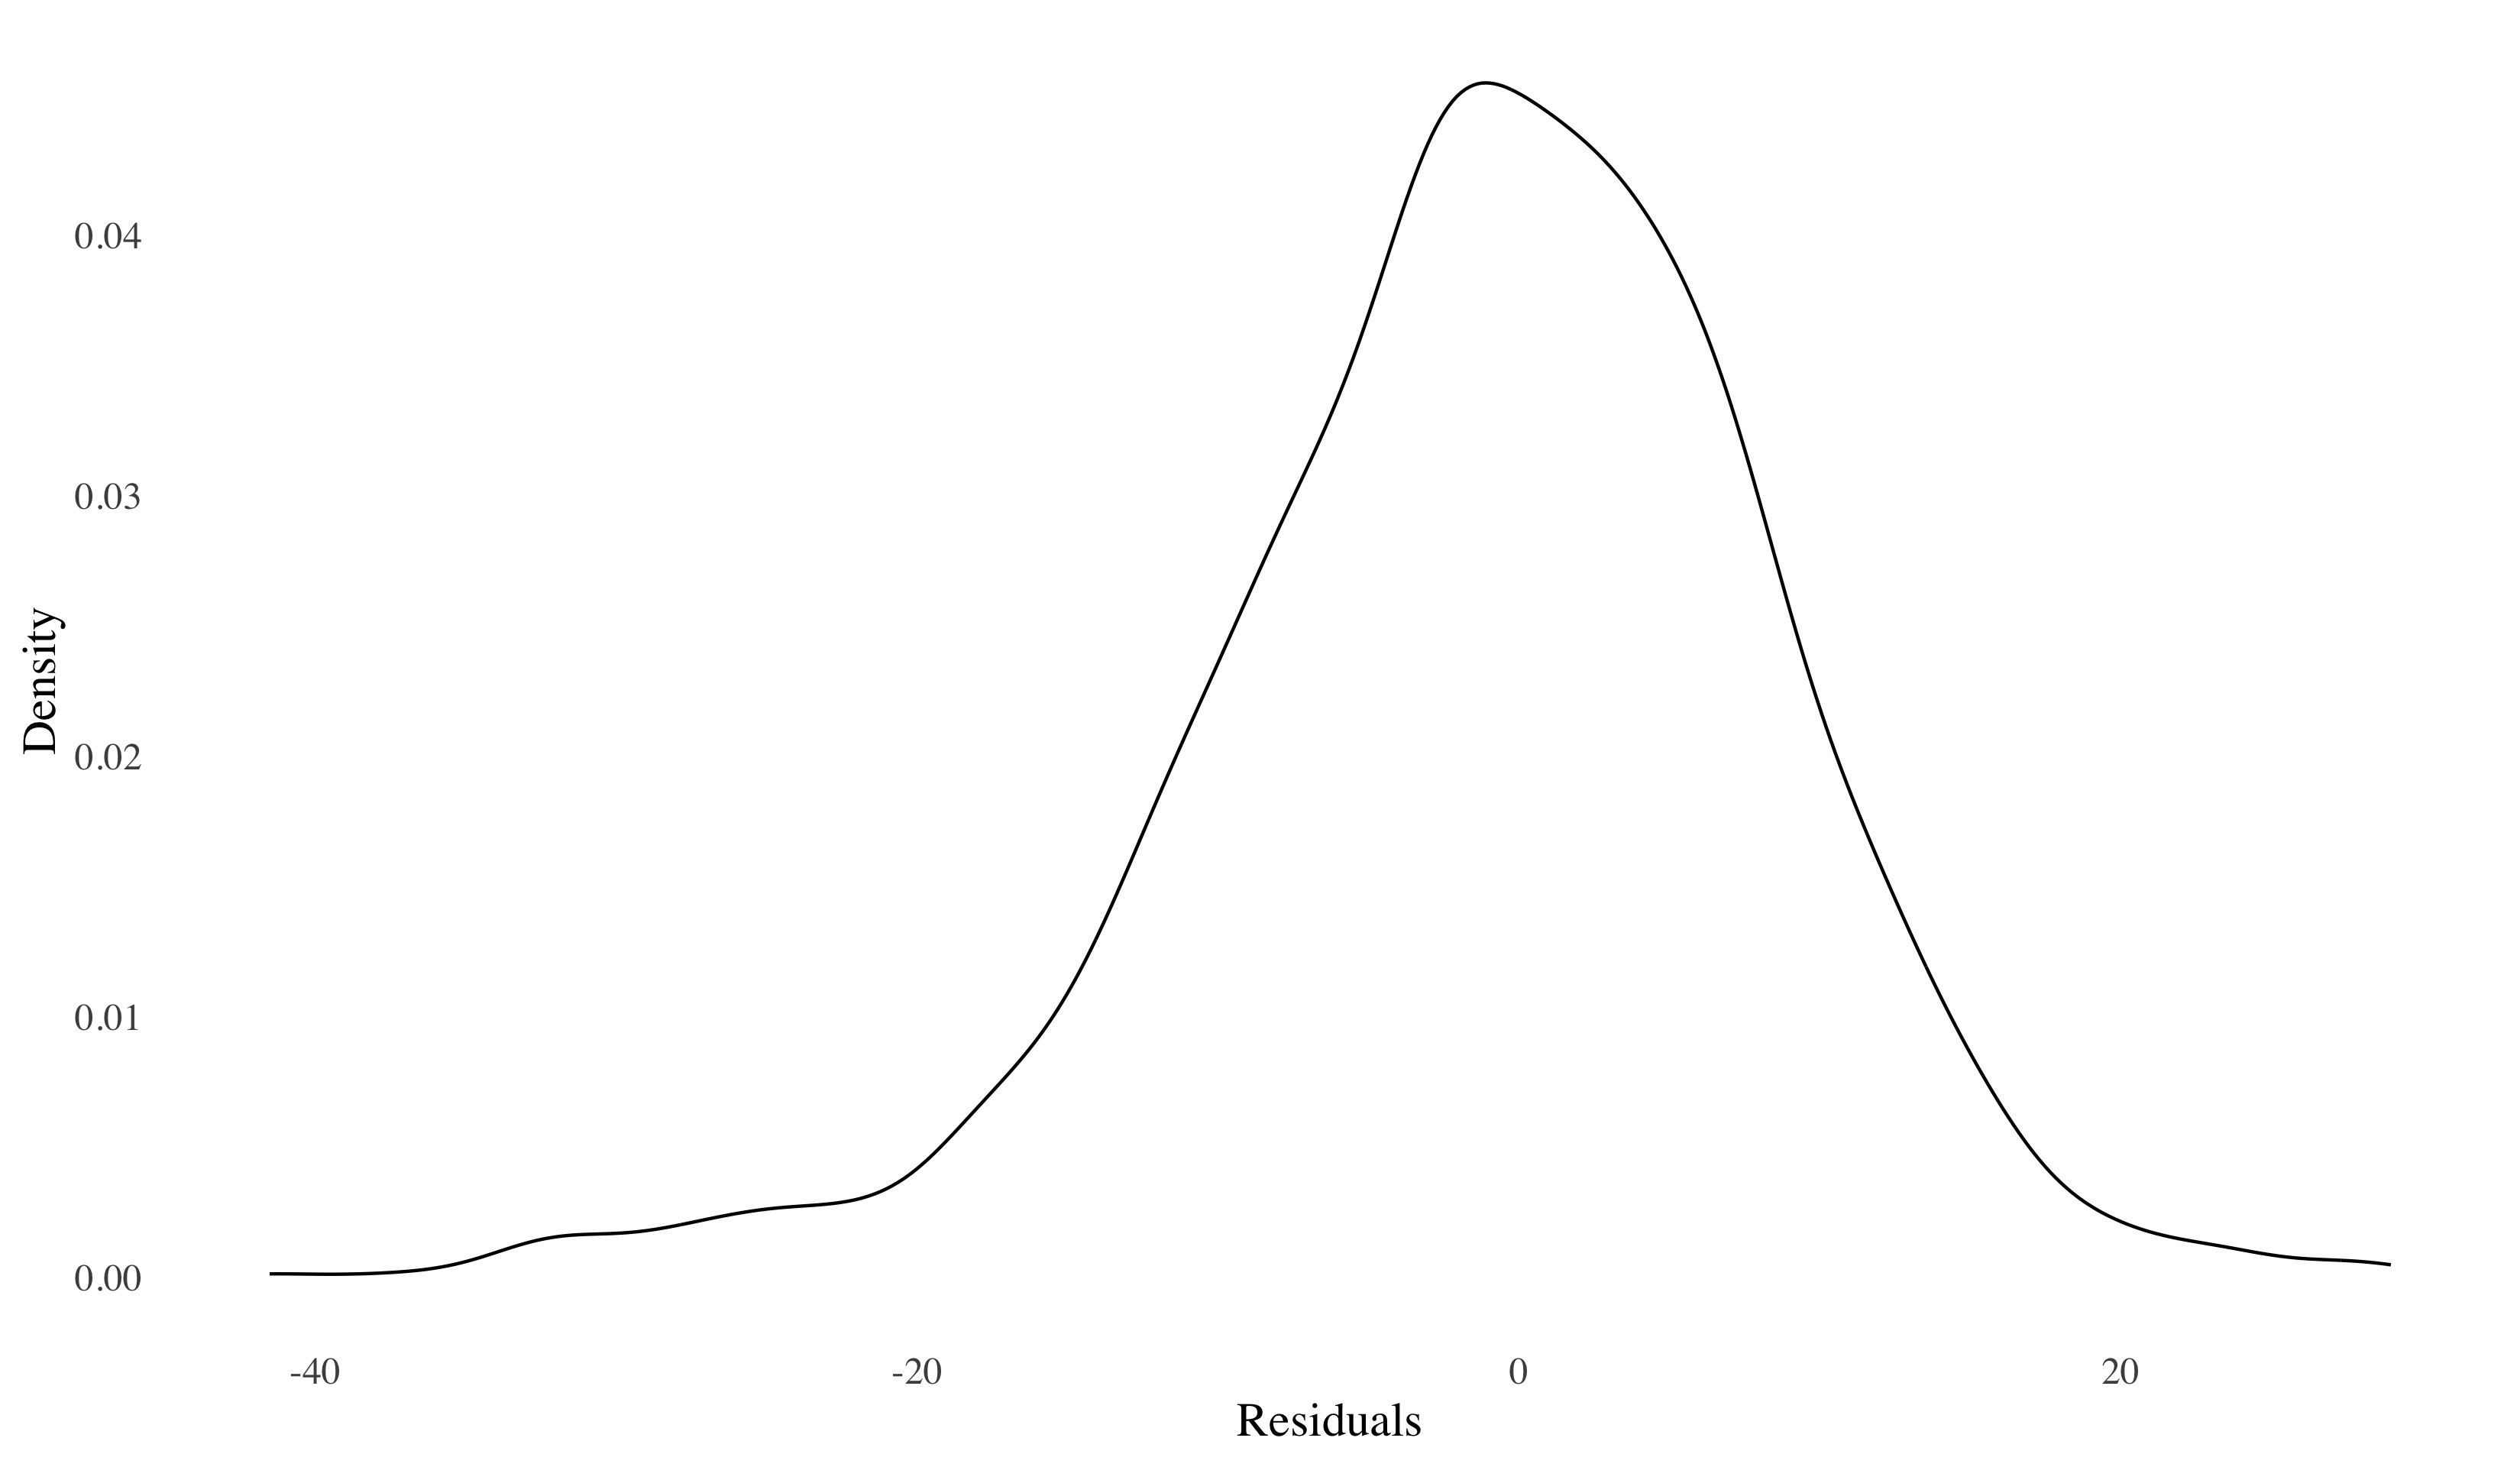
\includegraphics[scale = 0.14]{bayley_resids_plot}
\end{figure}

The Nurture data also feature intermittent missingness in Bayley composite scores throughout the study period. Of the total cohort (N = 666), 429 (64.4 \%) observations were available at three months, 435 (65.3 \%) observations were available at six months, 418 (62.8 \%) observations were available at nine months, and 437 (65.6 \%) observations were available at twelve months. As such, we require a modeling framework capable of dealing with missing data. 


\section{Model}
\label{s:model}

\subsection{Multivariate Skew Normal Mixture Model}

A primary goal of the Nurture study is to identify clusters of infants characterized by distinct motor development trajectories throughout the first year of life. To address this aim, we propose a flexible finite mixture model that accommodates relevant features of the data, such as skewness and dependence among the responses. For $i = 1,...,n$, let $\mathbf{y}_{i}=(y_{i1},\ldots,y_{iJ})^T$ be a $J \times 1$ vector of responses (i.e., Baley composite scores) for subject $i$ across the $J$ measurement occasions. For the analysis of the Nurture data, we propose a finite mixture model of the form
\begin{equation}
	\label{eq:mixture}
f(\mathbf{y}_i) = \sum_{k = 1}^{K} \pi_{ki} f(\mathbf{y}_i|\boldsymbol\theta_k),
\end{equation}
where $\boldsymbol\theta_k$ is the set of parameters specific to cluster $k$ ($k = 1,...,K$) and $\pi_{ki}$ is a subject-specific mixing weight representing the probability that subject $i$ belongs to cluster $k$. For now we assume that $K$ is fixed; in Section 4, we discuss model selection strategies for choosing the optimal value of $K$. 

To facilitate posterior inference, we introduce a latent cluster indicator variable $z_i$ taking the value $k \in \{1,...,K\}$ with probability $\pi_{ik}$. Conditional on $z_i = k$, we assume $\mathbf{y}_{i}$ is distributed as
\begin{equation}
\mathbf{y}_{i}|(z_i=k) \sim \text{MSN}_J(\boldsymbol\zeta_{ki},\boldsymbol\alpha_k,\boldsymbol\Omega_k), \label{eq:msndens}
\end{equation}
where $\text{MSN}_J(\cdot)$ denotes the $J$-dimensional multivariate skew normal density, $\boldsymbol\zeta_{ki}$ is a $J \times 1$ vector of subject- and cluster-specific location parameters, $\boldsymbol\alpha_k$ is a $J \times 1$ vector of cluster-specific skewness parameters, and $\boldsymbol\Omega_k$ is a $J \times J$ cluster-specific scale matrix that captures dependence among the $J$ responses for subject $i$. The vector $\boldsymbol\alpha_k$ has components $\alpha_{kj}$, $j = 1,...,J$, that control the skewness of outcome $j$ in cluster $k$. When $\boldsymbol\alpha_k = \mathbf{0}$, the MSN distribution reduces to the multivariate normal distribution $\text{N}_J(\boldsymbol\zeta_{ki},\boldsymbol\Omega_k)$, where $\boldsymbol\zeta_{ki}$ is a $J \times 1$ mean vector and $\boldsymbol\Omega_k$ is a $J \times J$ covariance matrix (Azzalini and Dalla Valle, 1996).

We can extend model (\ref{eq:msndens}) to the regression setting by modeling $\boldsymbol\zeta_{ki}$ as a function of covariates. Here we adopt a convenient stochastic representation of the MSN density (Azzalini and Dalla Valle, 1996):
\begin{equation}
\mathbf{y}_{i}|(z_i=k,t_i) = \mathbf{X}_i \boldsymbol\beta_k + t_i \boldsymbol\psi_k + \boldsymbol\epsilon_{ki}, \label{eq:msnreg}
\end{equation}
where 
$\mathbf{X}_i$ is a $J \times Jp$ design matrix that includes potential time-varying covariates (e.g., indicators denoting quarterly visits); $\boldsymbol{\beta}_k=(\beta_{k11},\ldots,\beta_{k1p},\ldots,\beta_{kJ1},\ldots,\beta_{kJp})^T$ is a $Jp\times 1$ vector of cluster- and outcome-specific regression coefficients; $t_i\sim \text{N}_{[0,\infty)}(0,1)$ is a subject-specific standard normal random variable truncated below by zero; $\boldsymbol\psi_k=(\psi_{k1},\ldots,\psi_{kJ})^T$ is a $J \times 1$ vector of cluster-specific skewness parameters; and $\boldsymbol{\epsilon}_{ki} \sim \text{N}_J(\boldsymbol0,\boldsymbol\Sigma_k)$ is a $J\times 1$ vector of correlated error terms. Thus, conditional on $t_i$ and $z_i=k$, $\boldsymbol{y}_i$ is distributed as $\text{N}_J(\mathbf{X}_i \boldsymbol\beta_k + t_i \boldsymbol\psi_k, \boldsymbol{\Sigma}_k)$. Marginally (after integrating over $t_i$), $\mathbf{y}_i|(z_i = k)$ is distributed $\text{MSN}_J(\boldsymbol\zeta_{ki}, \boldsymbol\alpha_k, \boldsymbol\Omega_k)$, where through back-transformation 
\begin{eqnarray}
\boldsymbol\zeta_{ki} &=& \mathbf{X}_i\boldsymbol\beta_k, \nonumber \\
\boldsymbol\alpha_k &=& \frac{1}{\sqrt{1 - \boldsymbol\psi_k^T 
\boldsymbol\Omega^{-1}_k\boldsymbol\psi_k}} \boldsymbol\omega_k \boldsymbol\Omega^{-1}_k\boldsymbol\psi_k,~~\text{and} \label{eqn:back_transform}\\
\boldsymbol\Omega_k &=& \boldsymbol\Sigma_k  + \boldsymbol\psi_k \boldsymbol\psi_k^T \nonumber,
\end{eqnarray}
where $\boldsymbol\omega_k = \text{Diag}(\boldsymbol\Omega_k)^{1/2}$ is the $J \times J$ diagonal matrix containing the square root of the diagonal entries of $\boldsymbol\Omega_k$. Additional details can be found in Fr\"{u}wirth-Schnatter and Pyne (2010). 

Of note, the MSN density can be expressed more compactly in terms of the matrix skew normal (MatSN) density (Chen and Gupta 2005). As we will see in Section 3.6, the matrix representation of the MSN distribution admits convenient conjugate prior distributions for the regression parameters and scale matrices, which in turn leads to efficient Gibbs sampling for posterior inference. Let $\mathbf{Y}_k$ be an ${n_k \times J}$ response matrix with rows $\mathbf{y}_i^T$, $(i = 1,...,n_k)$, where $n_k = \sum_{i = 1}^n {1}_{(z_i = k)}$ is the number of observations in cluster $k$. From equation (\ref{eq:msnreg}), it follows that $\mathbf{Y}_k$ is distributed as
\begin{eqnarray}
\mathbf{Y}_{k} &\sim& \text{MatSN}_{n_k \times J}(\mathbf{M}_k,\boldsymbol\alpha_k,\mathbf{I}_{n_k},\boldsymbol\Omega_k)\\
%\text{vec}(\mathbf{Y}_k) =  (\mathbf{y}^T_1,...,\mathbf{y}^T_{n_k})^T\\
\text{vec}(\mathbf{M}_k) &=& (\boldsymbol\zeta_{k1}^T,...,\boldsymbol\zeta_{kn_k}^T)^T, \nonumber
\end{eqnarray}
where $\boldsymbol\zeta_{ki} = \mathbf{X}_i \boldsymbol\beta_k$ as in equation (\ref{eq:msnreg}), $\boldsymbol\alpha_k = (\alpha_{k1},...,\alpha_{kJ})^T$, $\mathbf{I}_{n_k}$ is the $n_k\times n_k$ identity matrix, and $\boldsymbol\Omega_k$ is the $J\times J$ scale matrix defined above in equation (\ref{eq:msndens}). From equation (\ref{eq:msnreg}), it follows that $\mathbf{Y}_{k}$, conditional on the $n_k\times 1$ vector of random effects $\mathbf{t}_{k} = (t_1,...,t_{n_k})^T$, is jointly distributed in matrix form as
\begin{equation}
\mathbf{Y}_k | \mathbf{t}_k \sim \text{MatNorm}_{n_k \times J}(\mathbf{M}^*_k, \mathbf{I}_{n_k}, \boldsymbol\Sigma_k),
\end{equation}
where $\text{MatNorm}_{n_k \times J}(\cdot)$ denotes a $n_k\times J$ matrix normal density, $\text{vec}(\mathbf{M}^*_k) = \mathbf{X}_{k} \boldsymbol\beta_k + \mathbf{t}_k \otimes \boldsymbol\psi_k$ is an $n_kJ\times 1$ mean vector, $\mathbf{X}_k$ is an $n_kJ \times Jp$ design matrix, $\boldsymbol\beta_k$ is the $Jp\times 1$ vector of regression coefficients defined in equation (\ref{eq:msnreg}), and $\boldsymbol\Sigma_k$ is the $J\times J$ conditional covariance of $\boldsymbol\epsilon_{ik}$ given in equation (\ref{eq:msnreg}).

\subsection{Multinomial Regression for the Cluster Indicators}
To accommodate heterogeneity in the cluster-membership probabilities, we model $\pi_{ik}$ as a function of covariates using a multinomial logit model 
\begin{eqnarray}
\pi_{ik} = \Pr(z_i = k|\mathbf{w}_i) = \frac{\text{e}^{\mathbf{w}_i^T \boldsymbol\delta_k}}{\sum_{h = 1}^K \text{e}^{\mathbf{w}_i^T \boldsymbol\delta_{h}}},~ k=1,\ldots,K,
\end{eqnarray}
where $\mathbf{w}_i$ is an $r\times 1$ vector of subject-level covariates, $\boldsymbol\delta_k$ is a $r\times 1$ vector of regression parameters associated with membership in cluster $k$. For identifiability purposes, we fix the reference category $k = K$ and set $\boldsymbol\delta_K = \mathbf{0}$. Under this model, $z_i|\mathbf{w}_i \sim \text{Multinomial}(1,\boldsymbol\pi_i)$, where $\boldsymbol\pi_i = (\pi_{i1},...,\pi_{1K})$. During MCMC estimation, the cluster labels $z_i$ are updated from their multinomial full conditional distribution and used in the remaining MCMC steps as cluster assignments as detailed later in section (\textbf{what section}). By allowing the cluster probabilities to vary across subjects, our model can be viewed as a \textit{mixture of experts} model in which $\pi_{ki}$ acts as a \textit{gating function} controlling the prior probability of membership in cluster $k$, and $f(\mathbf{y}_i|\boldsymbol\theta_k)$ in Equation \ref{eq:mixture} is the ``expert'' (Bishop 2016). 

To facilitate sampling, we adopt an efficient data-augmentation approach introduced by Polson \textit{et al.} (2013), which expresses the inverse-logit function as a mixture P\'olya--Gamma densities. By using P\'olya--Gamma data augmentation for the multinomial model, we obtain a \textit{P\'olya--Gamma mixture of experts model}, a computationally efficient way to obtain inferences for the mixing weights in the Bayesian setting. A random variable ${w}$ is said to follow a P\'olya--Gamma distribution with parameters $b > 0$ and $c \in \mathbb{R}$ if
\begin{equation}
{w} \sim \text{PG}(b,c) \stackrel{d}{=} \frac{1}{2\pi^2}\sum_{s=1}^{\infty}\frac{g_s}{(s-1/2)^2 + c^2/(4\pi^2)}, \label{eq:pg1}
\end{equation}
where $g_s \stackrel{iid}{\sim} \text{Ga}(b,1)$ for $s = 1,...,\infty$ . Polson \textit{et al.} (2013) establish that for the $\text{PG}(b,c)$ density, and for $a,\eta \in \mathbb{R}$, 

\begin{equation}
\frac{(\text{e}^{\eta})^a}{(1 + \text{e}^{\eta})^b} = 2^{-b}\text{e}^{\kappa \eta} \int_{0}^{\infty} \text{e}^{-{w}\eta^2/2}p({w}|b,c = 0)d{w}. \label{eq:pg2}
\end{equation}
where $\kappa = a - b/2$. Polson \textit{et al.} also show that the conditional distribution $p(w|b,c)$ results from an ``exponential tilting'' of the $\text{PG}(b,0)$ density, thus

\begin{equation}
	p({w}|b,c) = \frac{\text{e}^{-c^2{w}/2}p({w}|b,0)}{E_{{w}}[\text{e}^{-c^2{w}/2}]} = \frac{\text{e}^{-c^2{w}/2}p({w}|b,0)}{\int_0^\infty \text{e}^{-c^2{w}/2}p({w}|b,0)d{w}}. \label{eq:pg3}
\end{equation}

To make use of P\'olya--Gamma data augmentation, we first write the full conditional distribution of $\boldsymbol\delta_k$ as the prior for $\boldsymbol\delta_k$ times the multinomial likelihood for all $z_i$. $$p(\boldsymbol\delta_k|\mathbf{U}_k,\boldsymbol\delta_{h \ne k}) \propto p(\boldsymbol\delta_k) \prod_{i = 1}^{n} \pi_{ki}^{U_{ki}}(1-\pi_{ki})^{1-U_{ki}},$$
where $p(\boldsymbol\delta_k)$ denotes the prior distribution of $\boldsymbol\delta_k$, $\mathbf{U}_k = (U_{k1},...,U_{kn})$, $U_{ik} = {1}_{(z_i = k)}$ is an indicator that subject $i$ belongs to cluster $k$, and $\pi_{ki}$ is defined as in Section 3.4. We can rewrite $\pi_{ki}$ as follows
$$\pi_{ki} = P(U_{ki} = 1) = \frac{\text{e}^{\mathbf{w}_i^T \boldsymbol\delta_k - {c}_{ki}}}{1 + \text{e}^{\mathbf{w}_i^T \boldsymbol\delta_k - {c}_{ki}}} = \frac{\text{e}^{\eta_{ki}}}{1 + \text{e}^{\eta_{ki}}}$$
where ${c}_{ik} = \log \sum_{h \ne k} \text{e}^{\mathbf{w}_i^T \boldsymbol\delta_{h}}$ and $\eta_{ik} = \mathbf{w}_i^T \boldsymbol\delta_k - {c}_{ki}$. We note that the sum $\sum_{h \ne k} \text{e}^{\mathbf{w}_i^T \boldsymbol\delta_{h}}$ includes the reference category, but since we fix $\boldsymbol\delta_K = \mathbf{0}$, we have $\text{e}^{\mathbf{w}_i^T \boldsymbol\delta_K} = 1$, and hence
$$c_{ki} = \log \sum_{h \ne k} \text{e}^{\mathbf{w}_i^T \boldsymbol\delta_{h}} = \log \left ( 1 + \sum_{h \notin \{k,K \}} \text{e}^{\mathbf{w}_i^T \boldsymbol\delta_{h}} \right )^T$$. 
We can use these quantities to re-express the full conditionals for $\boldsymbol\delta_k$ as
\begin{eqnarray}
	p(\boldsymbol\delta_k|\mathbf{U}_k,\boldsymbol\delta_{h \ne k}) &\propto& p(\boldsymbol\delta_k) \prod_{i = 1}^{n} \left (\frac{\text{e}^{\eta_{ki}}}{1 + \text{e}^{\eta_{ki}}} \right )^{U_{ki}} \left (\frac{1}{1 + \text{e}^{\eta_{ki}}} \right )^{1-U_{ki}} \nonumber\\ &=& p(\boldsymbol\delta_k) \prod_{i = 1}^n \frac{(\text{e}^{\eta_{ki}})^{U_{ki}}}{1 + \text{e}^{\eta_{ki}}} \label{eq:pglogit}
\end{eqnarray}
which is essentially a logistic regression likelihood. We can thus apply the P\'olya--Gamma sampler described in Polson et al. (2013) for logistic regression to update each $\boldsymbol\delta_k$ one at a time based on the binary indicators $U_{ki}$. To accomplish this, we first define for $k = 1,...,k$, the $n \times 1$ vector $\mathbf{U}^*_{k} = \left( \frac{U_{k1}-1/2}{w_{k1}},...,\frac{U_{kn}-1/2}{w_{kn}} \right )^T$. Polson et al. (2013) show that, conditional on $\boldsymbol{w} = (w_{k1},...,w_{kn})^T$, $\mathbf{U}^*_{k}$ follows a $\text{N}_n (\boldsymbol\eta_k,\mathbf{O}_k^{-1})$ distribution with mean $\boldsymbol\eta_k = (\eta_{k1},...,\eta_{kn})^T$ and precision matrix $\mathbf{O}_k = \text{Diag}(w_{k1},...,w_{kn})$. Thus, it follows that the full conditional distribution of $\boldsymbol\delta_k$ is given by 
\begin{equation}
	p(\boldsymbol\delta_k|\mathbf{z},\mathbf{W}, \mathbf{O}_k) \propto p(\boldsymbol\delta_k) \text{exp} \left [ - \frac{1}{2} (\mathbf{U}^*_k - \mathbf{W}\boldsymbol\delta_k)^T \mathbf{O}_k (\mathbf{U}^*_k - \mathbf{W}\boldsymbol\delta_k)\right].
\end{equation}
By assuming a normal prior for $\boldsymbol\delta_k$, as detailed in Section 3.4, the full conditional distribution for $\boldsymbol\delta_k$ is normal with parameters that follow standard forms, which we provide in Section (\textbf{what section}).
\subsection{Conditional MSN Imputation}
To accommodate missing at random (MAR) responses, we propose a convenient imputation algorithm that can be implemented ``online'' as part of the Gibbs sampler. In Section 6, we discuss extensions to allow for non-ignorable missingness (i.e. observations missing not at random). Suppose $\mathbf{y}_i$ has $q_i\in (1,\ldots,J)$ observed values, denoted $\mathbf{y}^{obs}_i$, and $J-q_i$ intermittent missing values, denoted $\mathbf{y}^{miss}_i$. We can make use of the stochastic representation given in equation (\ref{eq:msnreg}) to impute $\mathbf{y}^{miss}_i$ from its conditional multivariate normal distribution given $(z_i,t_i,\mathbf{y}^{obs}_i)$:
\begin{eqnarray}
\mathbf{y}^{miss}_i|(z_i=k,t_i,\mathbf{y}^{obs}_i)&\sim& \text{N}_{J-q_i}(\boldsymbol\mu^{cond}_{ki},\boldsymbol\Sigma^{cond}_k),~\text{where}\nonumber\\
\boldsymbol\mu^{cond}_{ki}&=& \boldsymbol\mu^{miss}_{ki} + \boldsymbol\Sigma_{k12} \boldsymbol\Sigma_{k22}^{-1}(\mathbf{y}^{obs}_i - \boldsymbol\mu^{obs}_{ki}) \label{eq:impute}\\
\boldsymbol\Sigma^{cond}_k&=& \boldsymbol\Sigma_{k11} - \boldsymbol\Sigma_{k12}\boldsymbol\Sigma_{k22}^{-1}\boldsymbol\Sigma_{k21},\nonumber \\
\boldsymbol\mu_{ki} &=& \begin{pmatrix} \boldsymbol\mu_{ki}^{miss} \\ \boldsymbol\mu_{ki}^{obs} \end{pmatrix}, \ \text{and} \nonumber \\
\boldsymbol\Sigma_k &=& \begin{pmatrix} 
	\boldsymbol\Sigma_{k11} & \boldsymbol\Sigma_{k12}\\
	\boldsymbol\Sigma_{k21} & \boldsymbol\Sigma_{k22}
\end{pmatrix}, \ \text{where} \nonumber
\end{eqnarray}
$\boldsymbol\Sigma_{k11}$ is a $(J-q_i) \times (J-q_i)$ matrix containing the rows and columns of $\boldsymbol\Sigma_k$ corresponding to inicies of $\mathbf{y}_{i}$ where missingness occurs. Similarly, $\boldsymbol\Sigma_{k12}$ is a $(J-q_i) \times q_i$ matrix containing the rows of $\boldsymbol\Sigma_k$ that correspond to missing indices of $\mathbf{y}_i$, but columns of $\boldsymbol\Sigma_k$ that correspond to observed indices of $\mathbf{y}_i$. The remaining partitions $\boldsymbol\Sigma_{k21}, \ \text{and} \ \boldsymbol\Sigma_{k22}$ are defined in the same manner. Likewise, $\boldsymbol\mu_{ki} = \mathbf{X}_i \boldsymbol\beta_k$ is partitioned into $\boldsymbol\mu_{ki}^{miss}$ and $\boldsymbol\mu_{ki}^{obs}$ with respect to the missing and observed indices of $\mathbf{y}_i$, respectively. These results follow from conventional multivariate normal theory, which we detail in the Web Appendix. An attractive feature of this imputation algorithm is that it avoids multiplicative run-time scaling in $m$, the number of imputations (Gelman \textit{et al.} 2013; Zhou and Reiter, 2010). Our approach also provides more opportunities to explore the missing data parameter space than does multiple imputation, since missing values are drawn at each MCMC iteration, and often in practice $n_{sim} >> m$, where $n_{sim}$ is the number of MCMC iterations (\textbf{find a reference}). In Section 4, we conduct simulation studies to demonstrate that imputing the missing MSN responses improves inferences over available-case analysis.

\subsection{Bayesian Inference}

\subsubsection{Prior Specification}
We adopt a fully Bayesian inferential approach and assign prior distributions to all model parameters. Conveniently, all parameters admit conditionally conjugate priors, which greatly improves posterior computation via a data-augmented Gibbs sampler. For the MSN model component, we adopt a conditionally independent prior structure for $\boldsymbol\beta_k$ and $\boldsymbol\Sigma_k$, where $p(\boldsymbol\beta_k,\boldsymbol\Sigma_k) = p(\boldsymbol\Sigma_k)p(\boldsymbol\beta_k|\boldsymbol\Sigma_k)$. We choose the normal-inverse-Wishart distribution for $p(\boldsymbol\beta_k,\boldsymbol\Sigma_k)$ by specifying $\boldsymbol\Sigma_k \sim \text{IW}(\mathbf{V}_{0k},\nu_{0k})$ and $\boldsymbol\beta_k|\boldsymbol\Sigma_k \sim \text{N}_{Jp}(\mathbf{b}_k,\mathbf{I}_p \otimes \boldsymbol\Sigma_k)$. We assign the skewness coefficients $\boldsymbol\psi_k$ a conjugate $\text{N}_J(\mathbf{m}_k,\mathbf{P}_k)$ prior. In practice, the updates of $\boldsymbol\beta_k$ and $\boldsymbol\psi_k$ can be combined into one step by defining the $(Jp + J) \times 1$ vector $\boldsymbol\beta^*_k = (\boldsymbol\beta_k^T,\boldsymbol\psi_k^T)^T$ for which we assume a $\text{N}_{Jp+J}(\mathbf{b}^*_k,\mathbf{I}_{(p+1)} \otimes \boldsymbol\Sigma_k)$ prior, where $\mathbf{b}^*_k$ is formed by concatenating $\mathbf{b}_k$ and $\mathbf{m}_k$. 

To make use of the Matrix Normal representation introduced previously in Section (\textbf{what section}), we define the matrix of regression parameters $\mathbb{B}^*_k$, where $\text{vec}(\mathbb{B}^*_k) = \boldsymbol\beta^*_k$. We assign $\mathbb{B}^*_k|\boldsymbol\Sigma_k$ a $\text{MatNorm}(\mathbf{B}^*_{0k},\mathbf{I}_{p+1},\boldsymbol\Sigma_k)$ prior, where $\mathbf{B}^*_{0k}$ is a matrix of location parameters such that $\text{vec}(\mathbf{B}^*_{0k}) = \mathbf{b}^*_k$, $\mathbf{I}_{p+1}$ is the identity matrix of dimensions $(p+1)\times(p+1)$, and $\boldsymbol\Sigma_k$ controls the correlation of the model error. This prior structure allows for convinient Matrix Normal updates of the MSN regression parameters as described in Section (\textbf{what section}).

For the multinomial logit model component, the regression parameters $\boldsymbol\delta_k = (\delta_{k1},...,\delta_{kr})$ are assigned a $\text{N}_r(\mathbf{d}_{0k}, \mathbf{S}_{0k})$ prior for $k = 1,...,K-1$, which is conditionally conjugate as described in Section (\textbf{what section}). We allow the normal-inverse-Wishart and multinomial hyperparameters to vary across clusters, though they may be shared across clusters in practice. An advantage of allowing for cluster-specific prior parameters is that \textit{a priori} knowledge of motor development trends can be incorporated into certain clusters while allowing the priors for other clusters to be less informative. Additionally, prior information regarding the effect of certain covariates on cluster membership can be incorporated in to the model by choosing informative values for $\mathbf{d}_{0k} \ \text{and} \ \mathbf{S}_{0k}$

\subsubsection{Posterior Inference} 
The above prior specification induces closed-form full conditionals that can be efficiently updated as part of a Gibbs sampler outlined below. A programatic sketch of our MCMC algorithm is given in Table (\ref{alg:MCMC}). Additional details, including derivations of full conditionals and MCMC diagnostics can be found in the Web Appendix. 

\paragraph{\textbf{Step 1}: Conditional MSN Imputation} The sampler begins with imputing missing values $\mathbf{y}_i^{miss}$ conditional on current  values of $z_i = k$ and $t_i$ as well as the associated $\mathbf{y}_i^{obs}$ observed data vector. This is accomplished by drawing $\mathbf{y}_i^{miss}$ from $\text{N}_{J-q_i}(\boldsymbol\mu^{cond}_{ki},\boldsymbol\Sigma^{cond}_k)$ as described in equation \ref{eq:impute} for all $i = 1,...,n$. Conditional imputation concludes with construction of a complete outcome vector $\mathbf{y}_i$ by merging the now imputed $\mathbf{y}_i^{miss}$ with $\mathbf{y}_i^{obs}$ with respect for the original ordering of the elements of $\mathbf{y}_i$.

\paragraph{\textbf{Step 2:} Update of MSN Regression Parameters} We begin the update of MSN regression parameters by updating $t_i$, the truncated Normal random effect used in the stochastic representation of $\mathbf{y}_i$ given in equation \ref{eq:msnreg}. For cluster $k$, compute $A_k = (1 + \boldsymbol\psi_k^T \boldsymbol\Sigma^{-1}_k\boldsymbol
\psi_k)^{-1}$ according to current values of $\boldsymbol\psi_k$ and $\boldsymbol\Sigma_k$. Now, for $i = 1,...,n_k$, where $n_k$ is the number of members of cluster $k$ according to the current cluster labeling ${z}_1,...,{z}_n$, compute $a_i = A_k \boldsymbol\psi_k^T \boldsymbol\Sigma^{-1}_k(\mathbf{y}_i - \boldsymbol\zeta_{ik})$, where $\boldsymbol\zeta_{ik} = X_i \boldsymbol\beta_k$. Finally, update $t_i$ from $\text{N}_{[0,\infty)}(a_i, \mathbf{A}_k)$ (\textbf{put derivations in supplement}).  Repeat these updates for $k = 1,...,K$

The remaining MSN regression parameters are updated from their full conditionals as follows. For each cluster $k$ ($k = 1,...,K$) we update $\boldsymbol\Sigma_k$ from $\text{IW}(\nu_k,\mathbf{V}_k)$, where $\nu_k = \nu_{0k} + n_k$ and\begin{eqnarray}
	\mathbf{V}_k &=&  (\mathbf{Y}-\mathbf{X}^*_k \mathbf{B}^*_k)^T (\mathbf{Y}_k - \mathbf{X}^*_k \mathbf{B}^*_k)\nonumber \\
	 &+& (\mathbf{B}_k^* - \mathbf{B}^*_{0k})^T \mathbf{I}_{p+1}(\mathbf{B}^*_k - \mathbf{B}^*_{0k}) + \mathbf{V}_{0k}. \nonumber
\end{eqnarray}We then make use of the Matrix Normal representation introduced in Section 3.2 to draw $\mathbb{B}^*_k$ from a $\text{MatNorm}_{p+1,J}(\mathbf{B}_k^*,\mathbf{L}_k^{-1},\boldsymbol\Sigma_k)$ density, where $\text{vec}(\mathbb{B}^*_k) = \boldsymbol\beta^*_k = (\beta_{k11},...,\beta_{kJp},\psi_{k1},...,\psi_{kJ})^T$ and
\begin{eqnarray}
	\mathbf{B}^*_k &=& (\mathbf{X}^{*T}_k \mathbf{X}^*_k + \mathbf{I}_{p+1})^{-1} (\mathbf{X}^{*T}_k \mathbf{Y}_k + \mathbf{I}_{p+1} \mathbf{B}_{0k}) \nonumber \\
	\mathbf{L}^*_k &=& \mathbf{X}^{*T}_k \mathbf{X}^*_k + \mathbf{I}_{p+1}. \nonumber
\end{eqnarray}

\paragraph{\textbf{Step 3:}P\'olya--Gamma Data Augmentation for $z_i$} The sampler concludes with updates of the multinomial regression parameters $\boldsymbol\delta_k$, for $k = 1,...,K-1$, followed by updates of each latent cluster indicator $z_i$ $(i=1,\ldots,n)$ from its multinomial logit full conditional. First, we define $U_{ki} = {1}_{z_i = k}$ for $i = 1,...,n$ and $k = 1,...,K-1$. Next, we update ${w}_{ki}$ from a $\text{PG}(1,\eta_{ki})$ density, where $\eta_{ki} = \mathbf{w}_i^T \boldsymbol\delta_k - {c}_{ki}$, and ${c}_{ki} = \log \sum_{h \ne k} \text{e}^{\mathbf{w}_i^T \boldsymbol\delta_{h}}$. Next, define $U^*_{ki} = \frac{U_{ki} - 1/2}{{w}_{ki}}$ and let $\mathbf{U}^*_k = (U^*_{k1},...,U^*_{kn})^T$. Finally, for $k = 1,...,K-1$, update $\boldsymbol\delta_k$ from a $\text{N}_r(\mathbf{d}_k,\mathbf{S}_k)$ density, where $\mathbf{S}_k = (\mathbf{S}_{k0} + \mathbf{W}^T \mathbf{O}_k \mathbf{W})^{-1}$, $\mathbf{O}_k = \text{Diag}({w}_{k1},...,{w}_{kn})$,  $\mathbf{d}_k = \mathbf{S}_k (\mathbf{S}_{k0}\mathbf{d}_{k0} + \mathbf{W}^T \mathbf{O}_k \boldsymbol\gamma_k)$, and $\mathbf{W}$ is the $n \times r$ matrix of multinomial logit regression covariates such that the $i^{th}$ row of $\mathbf{W}$ is $\mathbf{w}_i$.

Lastly, we update $z_1,...,z_n$ by first computing $\boldsymbol\pi_i = (\pi_{1i},...,\pi_{Ki})$ as
$$\pi_{ik} = \frac{\text{e}^{\mathbf{w}_i\boldsymbol\delta_k}}{1 + \sum_{h=1}^{K-1} \text{e}^{\mathbf{w}_i\boldsymbol\delta_h}},$$ 
for $i = 1,...n$ and $k = 1,...,K$. We also compute according to the multivariate Normal density of $\mathbf{y}_i|t_i$ the probability $P(\mathbf{y}_i|\boldsymbol\zeta^*_{ki},\boldsymbol\Sigma_k)$, where $\boldsymbol\zeta^*_{ki} = \mathbf{x}_i^*\boldsymbol\beta^*_k$. We use these quantities to compute $\boldsymbol\upsilon_{i} = (\upsilon_{1i},...,\upsilon_{Ki})$, where  
$$\upsilon_{ik} = P(z_i = k|\mathbf{y}_i,\boldsymbol\zeta^*_i,\boldsymbol\Sigma_k) = \frac{\pi_{ik}P(\mathbf{y}_i|\boldsymbol\zeta^*_{ki},\boldsymbol\Sigma_k)}{\sum_{h = 1}^{K} \pi_{ih}P(\mathbf{y}_i|\boldsymbol\zeta^*_{hi},\boldsymbol\Sigma_h)}$$.
The cluster labels $z_i$ are updated from a $\text{Multinomial}(1,\boldsymbol\upsilon_i)$ density for $i = 1,...n$, thus concluding the Gibbs sampler.


\subsubsection{MCMC Algorithm}

See Table 1.

\begin{algorithm}
\caption{Gibbs Sampler}
\label{alg:MCMC}
\begin{algorithmic}
\small
\linespread{0.5}
    \State $\mathbf{Define} \ n_{iter};\  n_{burn}; \ K; \ \boldsymbol\theta_{init}; \ \boldsymbol\theta_0$
    \State $n_{sim} := n_{iter} - n_{burn}$
    \State $\boldsymbol\theta := \boldsymbol\theta_{init}$
    \For {$\iota = 1,...,n_{sim}$}
        \State \textsc{I. Conditional Imputation}
          \For {$ i = 1,...,n$}
            \State $\mathbf{Draw} \ \mathbf{y}_i^{miss} \ \text{from} \ N_q(\boldsymbol\mu_i^{miss}, \boldsymbol\Sigma_i^{miss})$
            \State $\mathbf{y}_i := \mathbf{y}_i^{miss} \cup \mathbf{y}_i^{obs}$
         \EndFor
        \State \textsc{II. MSN Regression}
          \For {$ k = 1,...,K$}
            \State $n_k := \sum_{i = 1}^n {1}_{z_i = k}$
            \For {$i_k = 1,...,n_k$}
              \State $\mathbf{Draw}\  t_i \ \text{from} \ N_{[0,\infty)}(a_i,A)$
            \EndFor
            \State $\mathbf{X^*}_k := $ \texttt{cbind}$(\mathbf{X}_k,\mathbf{t}_k)$
            \State $\mathbf{Draw} \ \mathbf{B^*}_k \ \text{from} \ \text{MatNorm}(\mathbf{B}_k,\mathbf{L}_k^{-1},\boldsymbol\Sigma_k)$
            \State $\mathbf{Draw} \ \boldsymbol\Sigma_k \ \text{from} \ \text{InvWish}(\nu_k, \mathbf{V}_k)$
          \EndFor
        \State \textsc{III. Multinomial Logit}
          \For {$i = 1,...,n$}
            \For {$k = 1,...,K$}
              \State $\pi_{ik} := P(z_i = k|\mathbf{w}_i,\boldsymbol\delta_k)$
              \State $p_{ik} := P(\mathbf{y}_i|\boldsymbol\beta_k^{*T} \mathbf{x}^*_i,\boldsymbol\Sigma_k)$
            \EndFor
            \State $\mathbf{p}_{z_i} := \frac{\mathbf{p}_i \circ \boldsymbol\pi_i}{\mathbf{p}_i \cdot \boldsymbol\pi_i}$
            \State $\mathbf{Draw} \ z_i \ \text{from} \ \text{Categorical}(\mathbf{p}_{z_i})$
            \For {$k = 1,...,K-1$}
              \State $\mathbf{Draw} \ \boldsymbol\delta_k \ \text{from} \ N(\mathbf{M},\mathbf{S})$
            \EndFor
          \EndFor
        \State $\boldsymbol\theta := \{\mathbf{B^*}, \boldsymbol\Sigma, \mathbf{Z}, \boldsymbol\delta \}$
        \State $\mathbf{Store} \ \boldsymbol\theta$
	  \EndFor
\end{algorithmic}
\end{algorithm}


\subsubsection{Assessment of MCMC Convergence}

We monitor conver convergence of our MCMC algorithm through the use of standard approaches such Geweke's (1992) Z-diagnostic. In simulation studies under realistic parameter settings, we observed relatively fast convergence of all MCMC chains (i.e. within 1,000 iterations).

\subsubsection{Label Switching}

A common challenge for Bayesian mixture models is the so-called ``label switching" problem, in which draws of cluster-specific parameters may be assigned to the wrong cluster at some point during the MCMC simulation, rendering summaries of class-specific parameters incoherent. After conducting simulation studies under a wide variety of realistic parameter settings, as detailed in Section 4, we found little evidence of label switching in posterior draws of $\mathbf{z}$. When label switching was observed, we implemented \textit{post hoc} relabling algorithms as described in Papastamoulis 2016 and implemented in the \texttt{label.switching} package in \texttt{R}.

\subsubsection{Model Fit Diagnostics and Specification of K}

For model fit diagnostics, we choose the WAIC statistic introduced by Watanabe (2010). To specify the number of cluster $K$, we follow Neelon and Chung (2016), who use WAIC to determine the optimal number of latent factors in a Bayesian latent factor zero-inflated Poisson model for the analysis of correlated and zero-inflated count data. In Section 6, we discuss possible extentions to other methods for choosing $K$.

\newpage

\section{Simulation Studies}
\label{s:sim}

\subsection{Simulation to Compare to Multivariate Normal}

Our first simulation study will be concerned with comarison of the MSN mixture model to a standard multivariate normal mixture model. Here, the primary goal is to validate our parameter estimation scheme in a setting that resembles our application to the Nurture data. Our secondary goal is to investigate to what degree allowing for skewness in outcome components reduces the number of mixture components necessary to estimate the marginal density. For the purposes of illustration, we consider the following generative model 
\begin{eqnarray}
	f(\mathbf{y}_i) = \sum_{k = 1}^3 \pi_{ki} f(\mathbf{y}_i | \boldsymbol\theta_k), \nonumber
\end{eqnarray}
where $\boldsymbol\theta_k$ is the set of parameters specific to cluster $k$, for $k \in \{1,2,3 \}$, and $\mathbf{y}_i | \boldsymbol\theta_k \sim \text{MSN}_4(\boldsymbol\zeta_{ki},\boldsymbol\alpha_k,\boldsymbol\Omega_k)$, where $\boldsymbol\zeta_{ki} = (\zeta_{ki1},\zeta_{ki2},\zeta_{ki3},\zeta_{ki4}) = \mathbf{x}_i \boldsymbol\beta_{k}$. We note from the above model specification that the number of clusters $K = 3$ and the number of measurement occasions $J = 4$. For the MSN regression model, we fit a main effect for time (i.e. measurement occasion) in addition to a baseline covariate, whose value does not vary with time, but whose effect does vary with time. Under this setting with $p = 2$ covariates, the design matrix $\mathbf{x}_i$ for subject $i$ and the matrix of regression coefficients for cluster $k$, $\mathbf{B}_k$ are structured as

\begin{eqnarray}
	\mathbf{x}_i = 
	\begin{bmatrix}
		1 & 0 & 0 & 0 & x_i & 0 & 0 & 0\\
		0 & 1 & 0 & 0 & 0 & x_i & 0 & 0\\
		0 & 0 & 1 & 0 & 0 & 0 & x_i & 0\\
		0 & 0 & 0 & 1 & 0 & 0 & 0 & x_i\\
	\end{bmatrix}, \ \text{and} \ 
	\mathbf{B}_k = 
	\begin{bmatrix}
		\beta_{k11} & \beta_{k12} \\
		\beta_{k21} & \beta_{k22} \\
		\beta_{k31} & \beta_{k32} \\
		\beta_{k41} & \beta_{k42} \\
	\end{bmatrix}, \nonumber
\end{eqnarray}
where $\text{vec}({\mathbf{B}_k}) = \boldsymbol\beta_k$. Thus, for subject $i$ in cluster $k$, the $J = 4$ measurements have location parameters given by

\begin{eqnarray}
	\zeta_{ki1} &=& \beta_{k11} + \beta_{k12}x_i \nonumber \\
	\zeta_{ki2} &=& \beta_{k21} + \beta_{k22}x_i \nonumber \\
	\zeta_{ki3} &=& \beta_{k31} + \beta_{k32}x_i \nonumber \\
	\zeta_{ki4} &=& \beta_{k41} + \beta_{k42}x_i. \nonumber \\
\end{eqnarray}

For cluster $k$, we can collect all observations $\mathbf{y}_i$ ($i = 1,...,n_k$) into the $n_k \times 4$ matrix $\mathbf{Y}_k$ and all covariates $\mathbf{x}_i$ into the $4n_k \times 8$ matrix $\mathbf{X}_k$ to utilize the matrix Normal model specification detailed in Section 3, which allows for simultaneous updates of all MSN regression parameters in cluster $k$. For the multinomial regression model component of this simulation, we model the class labels $z_i$ as a function of an intercept and one baseline covariate, thus $r = 2$. We leave the problem of missing data to simulation study \#2 and do not incorporate missing data into this simulation.  

For our second goal in this simulation, to compare model performance when skewness is accounted for skewness to model performance when skewness is ignored, we fit both the proposed MSN finite mixture model as well as a classic multivariate Normal finite mixture model to data generated from an MSN distribution. We evaluate model fit in terms of absolute difference of parameter estimates as well as WAIC. 



\subsection{Simulation to Compare Imputation Methods}

In our second simulation study, we compare our online conditional multivariate normal imputation method to standard Bayesian multiple imputation. 

\subsection{Simulation to Assess Sensitivity to Misspecified K}

\newpage

\section{Application}
\label{s:app}

\begin{itemize}

\item Include both time varying and non-time varying covariates for the within cluster covariate set. 

\end{itemize}

\newpage

\section{Discussion}
\label{s:discuss}


\begin{itemize}

\item Discuss how we handle non-ignorable missingness 

\item Discuss other label switching approaches

\item Discuss skew-t?

\end{itemize}

\begin{thebibliography}{}

\bibitem{ } Arellano‐-Valle RB, Azzalini A. On the unification of families of skew‐normal distributions. \textit{Scandinavian Journal of Statistics}. 2006 Sep;33(3):561-74.

\bibitem{ } Azzalini A. A class of distributions which includes the normal ones. \textit{Scandinavian journal of statistics}. 1985 Jan 1:171-8.

\bibitem{ } Azzalini, A. and Dalla Valle, A. (1996). The multivariate skew normal distribution. Biometrika 83, 715–726.

\bibitem{ } Bishop, CM. Pattern recognition and machine learning. Springer; 2006.

\bibitem{ } Chen JT, Gupta AK. Matrix variate skew normal distributions. \textit{Statistics}. 2005 Jun 1;39(3):247-53.

\bibitem{ } Neelon SE, \O stbye T, Bennett GG, Kravitz RM, Clancy SM, Stroo M, Iversen E, Hoyo C. Cohort profile for the Nurture Observational Study examining associations of multiple caregivers on infant growth in the Southeastern USA. \textit{BMJ Open}. 2017 Feb 1;7(2):e013939.

\bibitem{ } Franczak BC, Tortora C, Browne RP, McNicholas PD. Unsupervised learning via mixtures of skewed distributions with hypercube contours. \textit{Pattern Recognition Letters}. 2015 Jun 1;58:69-76.

\bibitem{ } Fr\"{u}hwirth-Schnatter S, Pyne S. Bayesian inference for finite mixtures of univariate and multivariate skew-normal and skew-t distributions. \textit{Biostatistics}. 2010 Jan 27;11(2):317-36.

\bibitem{ } Ganjali M, Baghfalaki T. A Bayesian shared parameter model for analysing longitudinal skewed responses with nonignorable dropout. \textit{International Journal of Statistics in Medical Research}. 2014 Apr 1;3(2):103.

\bibitem{ } Geweke, J. Evaluating the accuracy of sampling-based ap- proaches to calculating posterior moments. \textit{Bayesian Statistics} Vol. 4, J. M. Bernardo, J. Berger, A. P. Dawid, and A.F.M. Smith (eds), 169–193. 1992. Cambridge, U.K.: Oxford University Press.

\bibitem{ } Gelman A, Stern HS, Carlin JB, Dunson DB, Vehtari A, Rubin DB. Bayesian data analysis. \textit{Chapman and Hall/CRC}; 2013 Nov 27.

\bibitem{ } Gelman A, Hwang J, Vehtari A. Understanding predictive information criteria for Bayesian models. \textit{Statistics and Computing}. 2014 Nov 1;24(6):997-1016.

\bibitem{ } Holmes CC, Held L. Bayesian auxiliary variable models for binary and multinomial regression. \textit{Bayesian Analysis}. 2006;1(1):145-68.

\bibitem{ } Lagona F, Picone M. Model-based clustering of multivariate skew data with circular components and missing values. \textit{Journal of Applied Statistics}. 2012 May 1;39(5):927-45.

\bibitem{ } Lanza ST, Rhoades BL. Latent class analysis: an alternative perspective on subgroup analysis in prevention and treatment. \textit{Prevention Science}. 2013 Apr 1;14(2):157-68.

\bibitem{ } Lee SX, McLachlan GJ. Model-based clustering and classification with non-normal mixture distributions. Statistical Methods \& Applications. 2013 Nov 1;22(4):427-54.

\bibitem{ } Lee SX, Mclachlan GJ. On mixtures of skew normal and skew-$t$ distributions. \textit{Advances in Data Analysis and Classification}. 2013 Sep 1;7(3):241-66.

\bibitem{ } Lin TI, Wang WL, McLachlan GJ, Lee SX. Robust mixtures of factor analysis models using the restricted multivariate skew-t distribution. \textit{Statistical Modelling}. 2018 Feb;18(1):50-72.

\bibitem{ } Luo S, Lawson AB, He B, Elm JJ, Tilley BC. Bayesian multiple imputation for missing multivariate longitudinal data from a Parkinson's disease clinical trial. \textit{Statistical Methods in Medical Research}. 2016 Apr;25(2):821-37.

\bibitem{ } Melnykov V, Maitra R. Finite mixture models and model-based clustering. \textit{Statistics Surveys}. 2010;4:80-116.

\bibitem{ } Neelon B, Chung D. The LZIP: A Bayesian latent factor model for correlated zero‐inflated counts. Biometrics. 2017 Mar;73(1):185-96.

\bibitem{ } Papastamoulis, P (2016). label.switching: An R Package for Dealing with the Label Switching Problem in MCMC Outputs. \textit{Journal of Statistical Software}, 69(1), 1-24. doi:10.18637/jss.v069.c01

\bibitem{ } Polson NG, Scott JG, Windle J. Bayesian inference for logistic models using P\'olya –- Gamma latent variables. Journal of the American statistical Association. 2013 Dec 1;108(504):1339-49.

\bibitem{ } Tiao GC, Zellner A. On the Bayesian estimation of multivariate regression. \textit{Journal of the Royal Statistical Society}: Series B (Methodological). 1964 Jul;26(2):277-85.

\bibitem{ } Viroli C. Finite mixtures of matrix normal distributions for classifying three-way data. \textit{Statistics and Computing}. 2011 Oct 1;21(4):511-22.

\bibitem{ } Vrbik I, Mcnicholas PD. Parsimonious skew mixture models for model-based clustering and classification. \textit{Computational Statistics \& Data Analysis}. 2014 Mar 1;71:196-210.

\bibitem{ } Watanabe S. Asymptotic equivalence of Bayes cross validation and widely applicable information criterion in singular learning theory. \textit{Journal of Machine Learning Research}. 2010;11(Dec):3571-94.

\bibitem{ } Zeller CB, Cabral CR, Lachos VH. Robust mixture regression modeling based on scale mixtures of skew-normal distributions. \textit{Test}. 2016 Jun 1;25(2):375-96.

\bibitem{ } Zhou X, Reiter JP. A note on Bayesian inference after multiple imputation. \textit{The American Statistician}. 2010 May 1;64(2):159-63.

\end{thebibliography}

\section{Appendix}

Put your final comments here. 

%  The \backmatter command formats the subsequent headings so that they
%  are in the journal style.  Please keep this command in your document
%  in this position, right after the final section of the main part of 
%  the paper and right before the Acknowledgements, Supplementary Materials,
%  and References sections. 

\backmatter

%  This section is optional.  Here is where you will want to cite
%  grants, people who helped with the paper, etc.  But keep it short!

\section*{Acknowledgements}

%  If your paper refers to supplementary web material, then you MUST
%  include this section!!  See Instructions for Authors at the journal
%  website http://www.biometrics.tibs.org




%  Here, we create the bibliographic entries manually, following the
%  journal style.  If you use this method or use natbib, PLEASE PAY
%  CAREFUL ATTENTION TO THE BIBLIOGRAPHIC STYLE IN A RECENT ISSUE OF
%  THE JOURNAL AND FOLLOW IT!  Failure to follow stylistic conventions
%  just lengthens the time spend copyediting your paper and hence its
%  position in the publication queue should it be accepted.

%  We greatly prefer that you incorporate the references for your
%  article into the body of the article as we have done here 
%  (you can use natbib or not as you choose) than use BiBTeX,
%  so that your article is self-contained in one file.
%  If you do use BiBTeX, please use the .bst file that comes with 
%  the distribution.  In this case, replace the thebibliography
%  environment below by 
%
%  \bibliographystyle{biom} 
% \bibliography{mybibilo.bib}

% \appendix

%  To get the journal style of heading for an appendix, mimic the following.


\label{lastpage}

\end{document}
